\cleardoublepage\chapter{Simulator}\label{chap:simulator}
The simulator is written in \textsc{Matlab} and C with MEX-interface, and contains vehicle generator, traffic generator, sensor simulator, (network simulator), algorithms. It is built in modules and can easily be expanded to fit the application. The modular layout can be seen in Figure~\ref{fig:software}.

There are a number of interfaces to the simulator, two of them can be seen in Figures \ref{fig:screen1} and \ref{fig:screen2}.

\begin{figure}
\centering
  \begin{minipage}{1\linewidth}
  \centering
   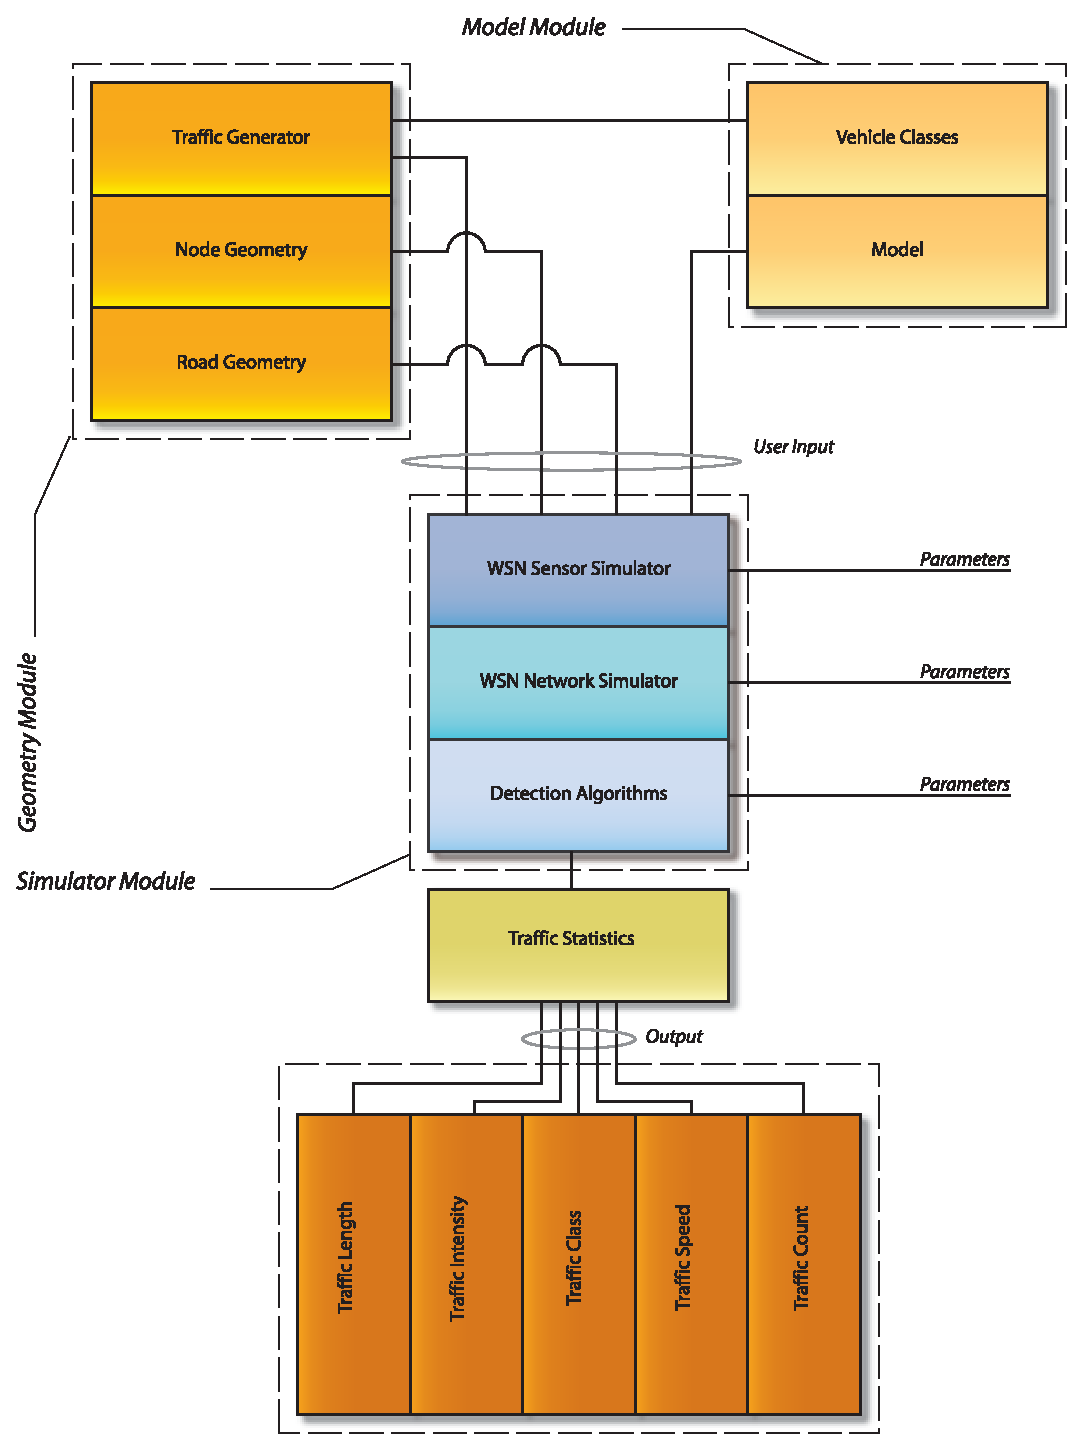
\includegraphics[width=1\linewidth]{images/software}
  \caption[Simulator overview]{Simulator overview. Modules.}
  \label{fig:software}
  \end{minipage}
\end{figure}

\begin{subfigures}
\begin{figure}
 \centering
 \begin{minipage}{0.8\linewidth}
 \centering
  % generated by laprint.m
% %
% \begin{psfrags}%
% \psfragscanon%
%
% text strings:
\psfrag{s05}[b][b]{\fontsize{8}{12}\fontseries{m}\mathversion{normal}\fontshape{n}\selectfont \setlength{\tabcolsep}{0pt}\begin{tabular}{c}Magnetic field strength [nT]\end{tabular}}%
\psfrag{s06}[t][t]{\fontsize{8}{12}\fontseries{m}\mathversion{normal}\fontshape{n}\selectfont \setlength{\tabcolsep}{0pt}\begin{tabular}{c}Time [s]\end{tabular}}%
\psfrag{s07}[b][b]{\fontsize{8}{12}\fontseries{m}\mathversion{normal}\fontshape{n}\selectfont \setlength{\tabcolsep}{0pt}\begin{tabular}{c}Magnetic field strength for different sensor yaw angle.\end{tabular}}%
\psfrag{s10}[][]{\fontsize{10}{15}\fontseries{m}\mathversion{normal}\fontshape{n}\selectfont \setlength{\tabcolsep}{0pt}\begin{tabular}{c} \end{tabular}}%
\psfrag{s11}[][]{\fontsize{10}{15}\fontseries{m}\mathversion{normal}\fontshape{n}\selectfont \setlength{\tabcolsep}{0pt}\begin{tabular}{c} \end{tabular}}%
\psfrag{s12}[l][l]{\fontsize{6}{12}\fontseries{m}\mathversion{normal}\fontshape{n}\selectfont $\alpha = 90^\circ$}%
\psfrag{s13}[l][l]{\fontsize{6}{12}\fontseries{m}\mathversion{normal}\fontshape{n}\selectfont $\alpha = 0^\circ$}%
\psfrag{s14}[l][l]{\fontsize{6}{12}\fontseries{m}\mathversion{normal}\fontshape{n}\selectfont $\alpha = 30^\circ$}%
\psfrag{s15}[l][l]{\fontsize{6}{12}\fontseries{m}\mathversion{normal}\fontshape{n}\selectfont $\alpha = 60^\circ$}%
\psfrag{s16}[l][l]{\fontsize{6}{12}\fontseries{m}\mathversion{normal}\fontshape{n}\selectfont $\alpha = 90^\circ$}%
%
% axes font properties:
\fontsize{6}{12}\fontseries{m}\mathversion{normal}%
\fontshape{n}\selectfont%
%
% xticklabels:
\psfrag{x01}[t][t]{-0.5}%
\psfrag{x02}[t][t]{0}%
\psfrag{x03}[t][t]{0.5}%
%
% yticklabels:
\psfrag{v01}[r][r]{-60}%
\psfrag{v02}[r][r]{-40}%
\psfrag{v03}[r][r]{-20}%
\psfrag{v04}[r][r]{0}%
\psfrag{v05}[r][r]{20}%
\psfrag{v06}[r][r]{40}%
%
% Figure:
% \resizebox{6cm}{!}{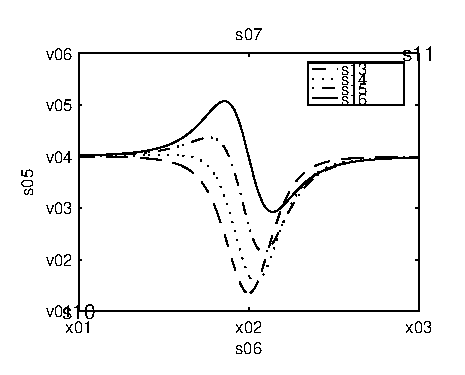
\includegraphics{xrotate.eps}}%
% \end{psfrags}%
%
% End xrotate.tex

  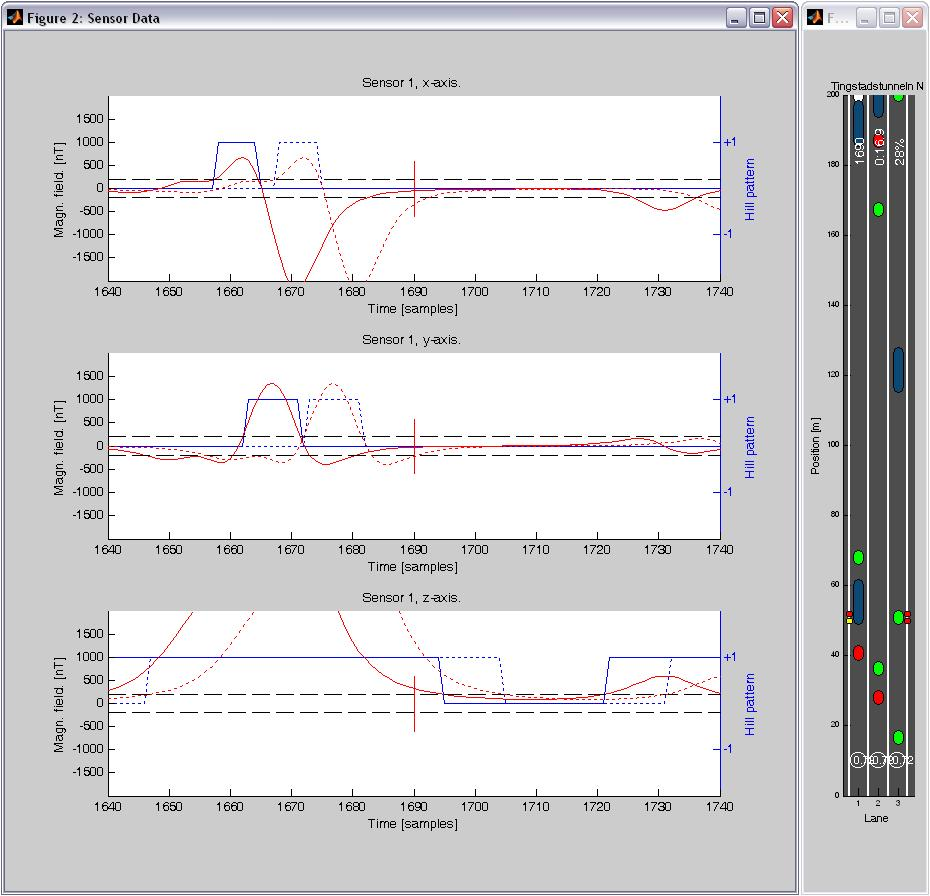
\includegraphics[width=1\linewidth]{images/screen1}
 % sensoraxis.eps: 1179666x1179666 pixel, 300dpi, 9987.84x9987.84 cm, bb=
 \caption[Simple simulator interface screenshot]{Simple simulator interface in \textsc{Matlab}.}
 \label{fig:screen1}
 \end{minipage}
 \end{figure}
 \begin{figure}
 \begin{minipage}{0.8\linewidth}
 \centering
 % % generated by laprint.m
% %
% \begin{psfrags}%
% \psfragscanon%
%
% text strings:
\psfrag{s05}[b][b]{\fontsize{8}{12}\fontseries{m}\mathversion{normal}\fontshape{n}\selectfont \setlength{\tabcolsep}{0pt}\begin{tabular}{c}Magnetic field strength [nT]\end{tabular}}%
\psfrag{s06}[t][t]{\fontsize{8}{12}\fontseries{m}\mathversion{normal}\fontshape{n}\selectfont \setlength{\tabcolsep}{0pt}\begin{tabular}{c}Time [s]\end{tabular}}%
\psfrag{s07}[b][b]{\fontsize{8}{12}\fontseries{m}\mathversion{normal}\fontshape{n}\selectfont \setlength{\tabcolsep}{0pt}\begin{tabular}{c}Magnetic field strength for different sensor pitch angle.\end{tabular}}%
\psfrag{s10}[][]{\fontsize{10}{15}\fontseries{m}\mathversion{normal}\fontshape{n}\selectfont \setlength{\tabcolsep}{0pt}\begin{tabular}{c} \end{tabular}}%
\psfrag{s11}[][]{\fontsize{10}{15}\fontseries{m}\mathversion{normal}\fontshape{n}\selectfont \setlength{\tabcolsep}{0pt}\begin{tabular}{c} \end{tabular}}%
\psfrag{s12}[l][l]{\fontsize{6}{15}\fontseries{m}\mathversion{normal}\fontshape{n}\selectfont $\beta = 90^\circ$}%
\psfrag{s13}[l][l]{\fontsize{6}{15}\fontseries{m}\mathversion{normal}\fontshape{n}\selectfont $\beta = 0^\circ$}%
\psfrag{s14}[l][l]{\fontsize{6}{15}\fontseries{m}\mathversion{normal}\fontshape{n}\selectfont $\beta = 30^\circ$}%
\psfrag{s15}[l][l]{\fontsize{6}{15}\fontseries{m}\mathversion{normal}\fontshape{n}\selectfont $\beta = 60^\circ$}%
\psfrag{s16}[l][l]{\fontsize{6}{15}\fontseries{m}\mathversion{normal}\fontshape{n}\selectfont $\beta = 90^\circ$}%
%
% axes font properties:
\fontsize{6}{15}\fontseries{m}\mathversion{normal}%
\fontshape{n}\selectfont%
%
% xticklabels:
\psfrag{x01}[t][t]{-0.5}%
\psfrag{x02}[t][t]{0}%
\psfrag{x03}[t][t]{0.5}%
%
% yticklabels:
\psfrag{v01}[r][r]{-100}%
\psfrag{v02}[r][r]{-50}%
\psfrag{v03}[r][r]{0}%
\psfrag{v04}[r][r]{50}%
\psfrag{v05}[r][r]{100}%
%
% % Figure:
% \resizebox{6cm}{!}{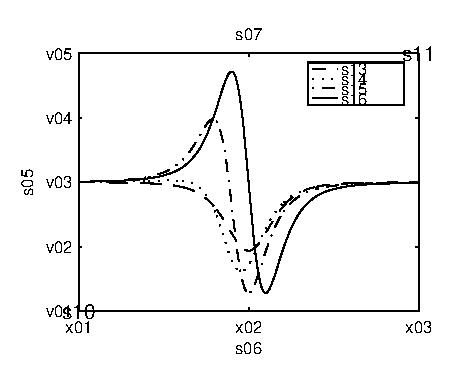
\includegraphics{zrotate.eps}}%
% \end{psfrags}%
% %
% End zrotate.tex

  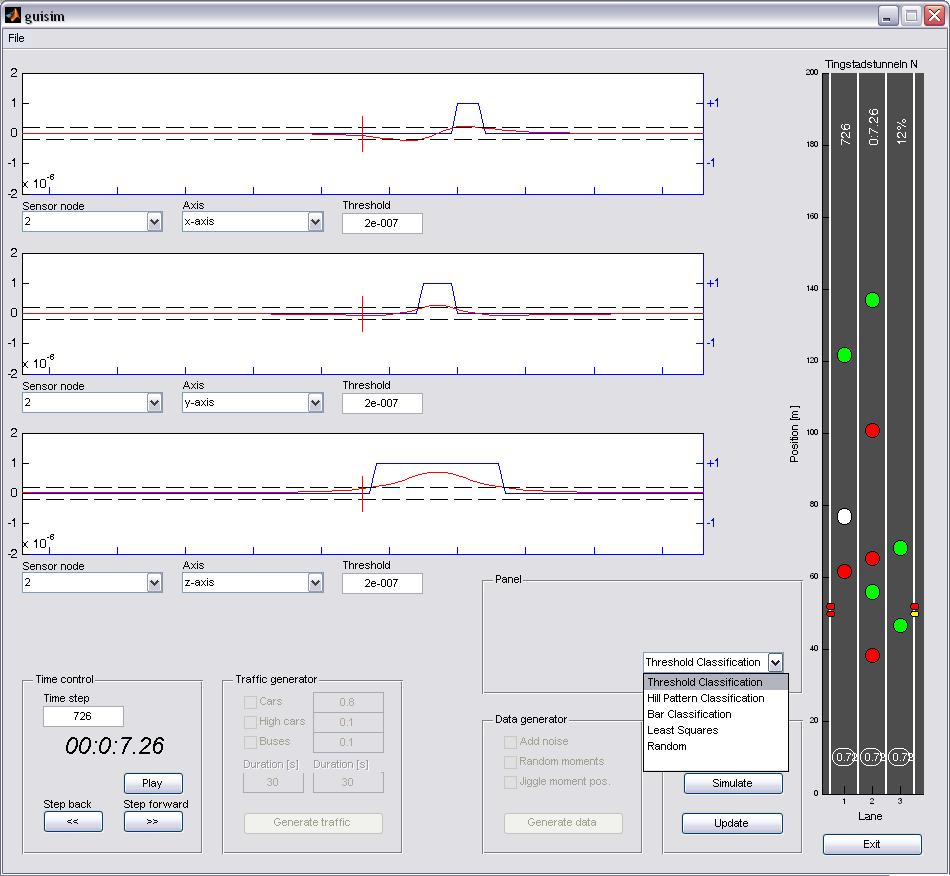
\includegraphics[width=1\linewidth]{images/screen2}
 % sensoraxis.eps: 1179666x1179666 pixel, 300dpi, 9987.84x9987.84 cm, bb=
 \caption[Advanced simulator interface screenshot]{Advanced simulator interface in \textsc{Matlab}.}
 \label{fig:screen2}
 \end{minipage}
\end{figure}
\end{subfigures}